\section{Auswertung}
\label{sec:Auswertung}
In der Auswertung wurden die Graphen in den Abbildungen 3 bis 6 mit Matplotlib \cite{matplotlib} und NumPy \cite{numpy} angefertigt.

\subsection{Bestimmung von RC mithilfe eines Entladevorgangs}
\begin{figure}[H]
	\centering
	\caption{Die Kondensatorspannung $U_C$ aus Tabelle 1 im Verlauf einer Entladung, sowie ihr Fit.}
	\includegraphics[width=\linewidth-70pt,height=\textheight-70pt,keepaspectratio]{graa.pdf}
	\label{fig:graa}
\end{figure}
\input{../build/taba.tex}

Mit der Beziehung $U_C = \frac{Q}{C}$ und Formel (5) ergibt sich:
\begin{displaymath}
ln(U_C) = -\frac{1}{RC}\cdot t + \ln U_0\text{.}
\end{displaymath}
Mithilfe einer linearen Ausgleichsrechnung der Form $y = mx+b$ ergibt sich mit den Wertepaaren ($\Delta t$, $\ln U_C$) aus Tabelle 1:
\begin{displaymath}
\tau = RC = -\frac{1}{m} = \SI{1.18 \pm 0.02}{\milli\second}\text{.}
%1,18 \text{ ms } \pm 0,02 \text{ ms.}
\end{displaymath}
\subsection{Bestimmung von RC mithilfe der Amplitudenfrequenzabhängigkeit}
\begin{figure}[H]
	\centering
	\caption{Amplituden aus Tabelle 2 in Frequenzabhängigkeit und der ermittelte Fit.}
	\includegraphics[width=\linewidth-70pt,height=\textheight-70pt,keepaspectratio]{grab.pdf}
	\label{fig:grab}
\end{figure}
\input{../build/tabb.tex}
Es werden $U_0$ und $\tau$ mit einer nichtlinearen Ausgleichsrechnung der Form $y = \frac{a}{\sqrt{1+(2\pi \cdot b\cdot x)^2}}$ mittels SciPy \cite{scipy} bestimmt. Es ergeben sich aus den Daten der Tabelle 2 und Formel (7):
\begin{displaymath}
U_0 = a = \SI{18.44 \pm 0.23}{\volt}
%U_0 = 18,44 \text{ V } \pm 0,23 \text{ V}
\end{displaymath}
und
\begin{displaymath}
\tau = RC = |b| = \SI{1.17 \pm 0.02}{\milli\second}\text{.}
%\tau = 1,17  \text{ ms } \pm 0,02 \text{ ms.}
\end{displaymath}

Es lässt sich erkennen, das zwischen dem $\tau$, berechnet aus den Daten der
 Teilaufgabe a) und dem aus denen von Teil b) nur ein sehr geringe Differenz
  besteht. Betrachtet man zudem die zugehörigen Fehler zeigt sich, dass die
	Differenz im Bereich der Messunsicherheit liegt. Dies lässt vermuten, dass höchstens ein geringer systematischer Fehler vorliegt.

\subsection{Bestimmung von RC mithilfe der Phasenverschiebung}
	 \begin{figure}[H]
	 	\centering
	 	\caption{Phasendifferenz $\varphi$ zwischen $U_{\text{Antrieb}}$ und $U_C$ aus Tabelle 3 in Abhängigkeit der Antriebsfrequenz mit ermittelten Fit.}
	 	\includegraphics[width=\linewidth-70pt,height=\textheight-70pt,keepaspectratio]{grac.pdf}
	 	\label{fig:grac}
	 \end{figure}
	 \input{../build/tabc.tex}
	 Es wird $\tau$ mithilfe einer nichtlinearen Ausgleichsrechnung der Form $y = \arctan(-2\pi \cdot a \cdot x)$ mittels SciPy \cite{scipy} bestimmt. Es ergibt sich aus den Daten aus Tabelle 3 mit Formel (8) und der Beziehung $\varphi=2\pi \cdot \Delta t \cdot f_{\text{Antrieb}}$ ohne Berücksichtigung der letzten 4 Werten, da bei hohen Frequenzen vermutlich Störeffekte auftreten:
	 \begin{displaymath}
	 \tau = RC = a = \SI{1.38 \pm 0.18}{\milli\second}\text{.}
	 %\tau = 1,38  \text{ ms } \pm 0,18 \text{ ms.}
	 \end{displaymath}


	 \subsection{Die RC-Kreis Relativamplitude in Abhängigkeit von der Phase}

	 \begin{figure}[H]
	  \centering
	  \caption{Amplitude $A$ als Relativamplitude, die Phasenverschiebung $\varphi$ aus Tabelle 4 und die Theoriekurve in einem Polarkoordinatensystem eingetragen.}
	  \includegraphics[width=\linewidth-70pt,height=\textheight-70pt,keepaspectratio]{grad.pdf}
	  \label{fig:grad}
	 \end{figure}
	 \input{../build/tabd.tex}
	 Mit der Formel (7) und Formel (8) ergibt sich:
	 \begin{equation}
	 A(\varphi) = U_0\cdot \sin(\varphi)\sqrt{\frac{1}{\sin^2(\varphi)}-1}\text{.}
	 \end{equation}
	 In diesem Polarkoordinantensystem werden die Theoriekurve, die durch Formel (12) gegeben ist und die Werte aus Tabelle 4 eingetragen. Der Winkel $\varphi$ ergibt sich aus den Werten für $\Delta t$ durch die Beziehung $\varphi=2\pi \cdot \Delta t \cdot f_{\text{Antrieb}}$ und die Relativamplitude ist $\frac{A}{U_{0}}$, wobei das in b) berechnete $U_{0}$ verwendet wurde. Die hohe systematische Abweichung muss in der Diskussion geklärt werden.



	 \subsection{Der RC-Kreis als Integrator}
	 \begin{figure}[H]
	 	\centering
	 	\caption{Zeitliche Verlauf von $U_0$ (gelb) und $U_C$ (blau) bei einer antreibenden Sinusspannung.}
	 	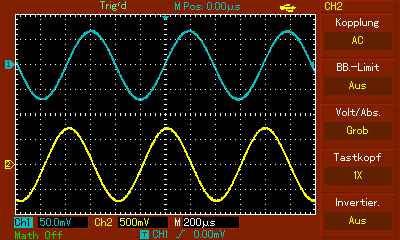
\includegraphics[width=\linewidth-70pt,height=\textheight-70pt,keepaspectratio]{content/MAP002.png}
	 	\label{fig:Sinus}
	 \end{figure}
	 In Abbildung 7 ist zu erkennen, dass die Spannung am Kondensator (blau) im Vergleich zur Spannung an der Spannungsquelle (gelb) um $\frac{\pi}{2}$ verschoben ist, was einer Integration der Sinus-Spannung an der Spannungsquelle mit einem Skalierungsfaktor entspricht.


	 \begin{figure}[H]
	 	\centering
	 	\caption{Zeitlicher Verlauf von $U_0$ (gelb) und $U_C$ (blau) bei einer antreibenden Dreieckspanung.}
	 	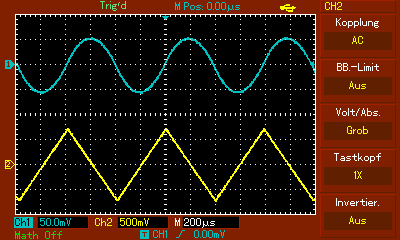
\includegraphics[width=\linewidth-70pt,height=\textheight-70pt,keepaspectratio]{content/MAP003.png}
	 	\label{fig:Dreieck}
	 \end{figure}
	 Auch bei Dreieckspannung an der Spannungsquelle (gelb) in Abbildung 8 lässt sich erkennen das die Spannung am Kondensator (blau) das Integral der Dreieckspannung ist, da die Kondensatorspannung sich wie bei einer Integration erwartet quardratisch verhält.

	 \begin{figure}[H]
	 	\centering
	 	\caption{Zeitliche Verlauf von $U_0$ (gelb) und $U_C$ (blau) bei einer antreibenden Rechteckspannung.}
	 	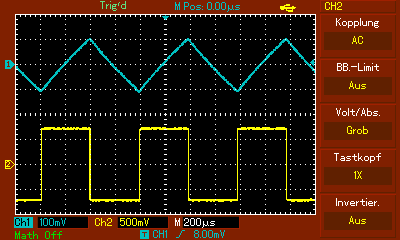
\includegraphics[width=\linewidth-70pt,height=\textheight-70pt,keepaspectratio]{content/MAP004.png}
	 	\label{fig:Rechteck}
	 \end{figure}
	 In Abbildung 9 beschreibt die Spannung an der Spannungsquelle eine Rechteckfunktion (gelb). Offensichtlich ist diese ein konstantes Vielfaches der Steigung der Kondensatorspannung (blau).\\

	 Diese Beobachtungen bestätigen die Vermutung, dass der RC-Kreis auch als Integrator genutzt werden kann.
